\documentclass[11pt]{article}
\usepackage[utf8]{inputenc}
\usepackage[T1]{fontenc}
\usepackage[final]{pdfpages} 
\usepackage[french]{babel}
\usepackage{amsmath}
\usepackage[bookmarks={true},bookmarksopen={true}]{hyperref}
\usepackage{graphicx}
\usepackage[a4paper]{geometry}
\usepackage{listings}
	\lstset{frame=tb,
		language=Java,
 		aboveskip=3mm,
  		belowskip=3mm,
  		showstringspaces=false,
  		columns=flexible,
  		basicstyle={\small\ttfamily},
  		numbers=none,
 		numberstyle=\tiny\color{gray},
  		keywordstyle=\color{blue},
  		commentstyle=\color{dkgreen},
  		stringstyle=\color{mauve},
  		breaklines=true,
  		breakatwhitespace=true
  		tabsize=3
	}
\pagestyle{plain}
\setlength{\parindent}{5mm}

\usepackage{color}

\definecolor{dkgreen}{rgb}{0,0.6,0}
\definecolor{gray}{rgb}{0.5,0.5,0.5}
\definecolor{mauve}{rgb}{0.58,0,0.82}



\title{\textbf{Projet LSINF1121 -  Algorithmique et structures de données\\ - \\ Rapport final Mission 3} \\ {\large Groupe 3.2}}
\author{Boris \bsc{Dehem} \\(5586-12-00)\and Sundeep \bsc{Dhillon} \\(6401-11-00)\and Alexandre \bsc{Hauet} \\ (5336-08-00) \and Jonathan \bsc{Powell}\\(6133-12-00)\and Mathieu \bsc{Rosar} \\ (4718-12-00)\and Tanguy \bsc{Vaessen} \\ (0810-14-00)}
\date{date}
\date{\vspace*{25mm}

\includegraphics[scale=0.75]{logo.jpg}\\
		\vspace*{30mm}
		\begin{center}
		Année académique 2014-2015 \\	
		\end{center}}

\begin{document}
\thispagestyle{empty}

\maketitle
\thispagestyle{empty}
%\tableofcontents
%\setcounter{tocdepth}{3}
%\setcounter{page}{1}
%\newpage
\section{Introduction}
Dans le cadre du cours "Algorithmique et structures de données", il nous a été demandé de concevoir et d’implémenter une application permettant d’accéder aux informations associées à une revue scientifique dont on fournit le nom. L’information principale est le rang de la revue dans le classement. Ce rang est représenté par un code : A*, A, B...etc.

\section{Choix d'implémentation}
Pour le choix du type de dictionnaire et son implémentation, le type \texttt{HashMap} de java fait exactement ce que l'on souhaite... Il utilise du Open Adressing, ce qui est le plus pratique. Il a déjà une fonction de compression, et comme la clé de noeuds entrées est leur titre, de type String, on utilise simplement la fonction \textit{hashCode} du type string.

\subsection{Diagramme de classes}
\begin{center}
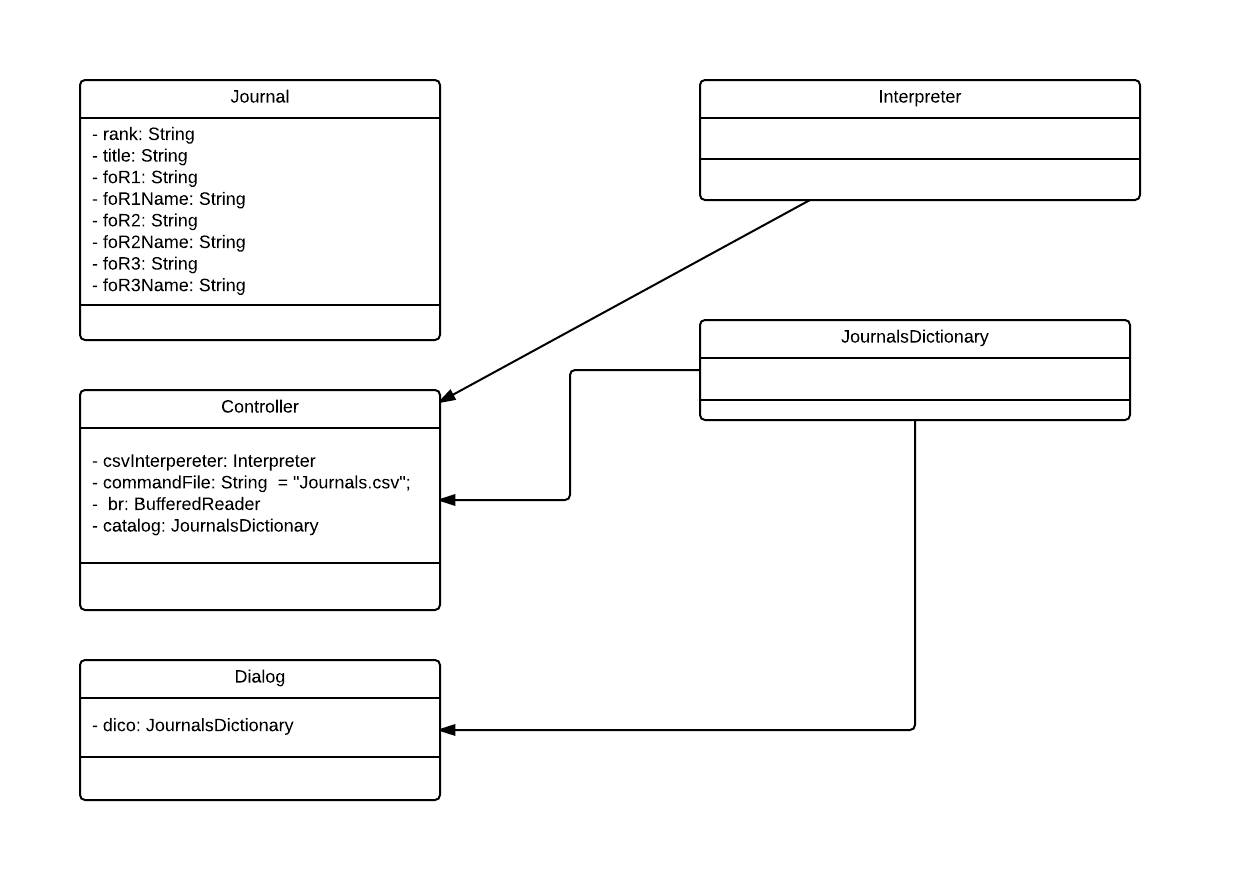
\includegraphics[scale=0.35]{diag.jpg}
\end{center}
\section{Analyse de la complexité calculatoire}

\subsection{Complexité temporelle}
\subsubsection*{Dans la classe Controller}
La méthode \texttt{interpreteFile()} de la classe \textit{Controller} est de complexité $\Theta$(n) avec n étant le nombre de lignes dans le fichier.

\section{Répartition du travail}

Rédaction du rapport : Alexandre et Sundeep. \\
Conception du programme : Boris, Jonathan, Sundeep et Tanguy, Mathieu.

\section{Difficultés rencontrées}
Grâce aux questions de la séance intermédiaire, nous avons décortiqué le problème ce qui nous a permis de préparer correctement le partie implémentation. Nous n'avons donc pas rencontré de réel problème lors de la partie développement du programme.

\end{document}